\documentclass[12pt,a4paper]{article}
\usepackage{graphicx}
\usepackage[nolist,nohyperlinks]{acronym}
\usepackage{tikz}
\usetikzlibrary{arrows,positioning, shapes}
\tikzset{
    %Define standard arrow tip
    >=stealth',
    %Define style for boxes
    drect/.style={
           rectangle,
           rounded corners,
           dashed,
           draw=black, thick,
           text width=6.5em,
           minimum height=2em,
           text centered},
   goval/.style={
          circle,
          draw=black, very thick,
          text width=6.5em,
          minimum height=2em,
          text centered},
    % Define arrow style
    pil/.style={
           ->,
           thick,
           shorten <=2pt,
           shorten >=2pt},
    arr/.style={
           ->,
           thick,
           shorten <=2pt,
           shorten >=2pt
           },
    dashedarr/.style={
            ->,
            thick,
            shorten <=2pt,
            shorten >=2pt,
            dashed
    }
}

\usepackage[numbers]{natbib}
\usepackage{float}
\usepackage{glossaries}
\usepackage[hyphens]{url}
% \usepackage[german]{babel}
\usepackage[british]{babel}
\usepackage[utf8]{inputenc} %für Umlaute äüöß
\usepackage{array}
\usepackage[bookmarks]{hyperref}
\graphicspath{{img/}}

\newpage
\section*{Abbreviations}
\begin        {acronym}[PowerTAC]
%:.,+33sort
	\acro {AI}       {artificial intelligence}
	\acro {CHP}      {combined heat and power unit}
	\acro {CLI}      {command-line interface}
    \acro {ReLu}     {rectified linear unit}
	\acro {CPU}      {central processing unit}
    \acro {MWh}      {megawatt hour}
	\acro {DU}       {distribution utility}
	\acro {DeepRL}   {deep reinforcement learning}
	\acro {GPU}      {graphical processing units}
	\acro {gRPC}     {Google remote procedure call}
	\acro {JAXB}     {Java architecture for XML}
	\acro {JMI}      {Java message service}
	\acro {JSON}     {Javascript object notation}
    \acro {kWh}      {killowatt hour}
	\acro {MDP}      {markovian decision process}
    \acro {A3C}      {asynchronous advantage actor-critic}
	\acro {POJO}     {plain old Java object}
	\acro {POMDP}    {partially observable markovian decision process}
	\acro {POPO}     {plain old Python object}
	\acro {PPO}      {proximal policy optimization}
	\acro {PowerTAC} {power trading agent competition}
    \acro {DDPG}     {deep deterministic policy gradient}
    \acro {DQN}      {deep Q network}
    \acro {NAF}      {normalized advantage function}
	\acro {RL}       {reinforcement learning}
	\acro {SARSA}    {state-action-reward-state-action}
	\acro {SOTA}     {state-of-the-art}
    \acro {SELF}     {smart electricity market learners with function approximation}
	\acro {TPU}      {tensor processing unit}
	\acro {XML}      {extensive markup language}
    \acro {API}      {application programming interface}
    \acro {CNN}      {convolutional neural network}
    \acro {CRIU}     {checkpoint/restore in userspace}
    \acro {LSTM}     {long short-term memory}
    \acro {RNN}      {recurrent neural networks}
    \acro {SSL}      {secure socket layers}
    \acro {UI}       {user interface}
    \acro {VM}       {virtual machine}

\end{acronym}



%\title{TODO Find best: Social Artificial Neural Network Learning\\
\title{Best-Peer Imitation in Groups of Reinforcement Learning Agents \\
\small{Expose for Master Thesis}}

\author{Pascal Brokmeier}

\begin{document}
\pagenumbering{arabic}
\maketitle

\section{Motivation}

% TEXT START
Artificial intelligence is one of the most discussed technology of the last years. Machine learning algorithms have recently been developed that allow computers to reliably classify many object classes in images \cite{krizhevsky2012imagenet} through supervised learning but also also allow robotics to employ reinforcement learning which let humanoids learn to walk reliably and even perform backflips \cite{proximalpolicyopt}.

There are also many economical motivations to advance the abilities of machine learning. From autonomous vehicle control such as cars or helicopters \cite{abbeel2010autonomous} to autonomous agents helping to balance the complex electricity grids of the future \cite{peters2013reinforcement} to already widely available technologies such as image classifications for consumer cloud storage or consumer recommendation engines for online advertising. Reinforcement learning specifically offers the ability to let machines perform complex operations without the need to provide thousands or sometimes millions of labeled examples as is often required for supervised learning methods. They also have been shown to quickly learn actions from only very few demonstrations which could allow humans to demonstrate an action that is then mimicked by a RF based agent \cite{duan2017one}.


Interestingly, most approaches, independent of the architecture of the neural network, approach the task of learning with one network in mind \cite[p.694ff]{russell2016artificial}. Yet, humans and animals exhibiting higher forms of intelligence as well as many low intelligence species learn in small to large groups or even swarms. Their knowledge is not only a product of individual intelligence but a result of complex network effects of many individuals influencing and interacting with each other \cite[p.200f]{sloman2017knowledge}.

\citeauthor{sloman2017knowledge} and \citeauthor{wegner1995computer} argue that intelligence, as seen in humans, must not only be attributed to the individual intelligence but is also caused due to a constant setting of social interaction between many individuals that lead to cultural and technical advancement because of an emergent \emph{community of knowledge}.

Humans have always distributed labor among many individuals and more importantly, humans distribute learning tasks to individuals. Everyone has a different learning history and specializes in different tasks. We then influence each others' way of thinking by interacting with each other and observing each other. This is true for children just as it is for complex academic communities. AI agent learning research has not approached the topic with similar environments, relying mostly on single agents or sometimes training a multitude of agents but then selecting the best ones and dismissing the rest, simply to increase the amount of samples which increase the chance of a well trained example to be found.

%Looking at the research of artificial intelligence, the field or reinforcement learning has long defined approaches towards finding a balance between agents that solely try to do as well as they can \emph{in the current iteration} and those that explore the state space to learn new approaches and solutions to reach higher utilities. Commonly, this is accomplished through a degenerating probability of making a \emph{less than optimal} choice when selecting an action, favoring those actions that lead to yet less explored states \cite[]{russel12016artificial}.

Finally, when looking at the complexity of AI algorithms and agent learning, time and performance constraints are always a key factor for viability of a theoretical algorithm. An algorithm that has exponential complexity in the number of states of the environment is usually only viable for small problems, only few of which can be found in real world problems \cite[p.839f.]{russel2016artificial}. While many algorithms are highly parallelizable \cite{tensorflow2015-whitepaper}, only the most recent incarnations of freely available software tools and libraries are capable of massive distribution of algorithms like proximal policy optimization across many GPU nodes \cite{hafner2017agents}. So as has long been a tradition in computer science, algorithms are only viable if they can either be expected to provide a solution in polynomial time or alternatively if they are easily parallelizable. Distribution of human labor in societies can be viewed as the equivalent to multi-threaded execution of algorithms in computers.

\section{Research question and possible results}

Based on the previously enumerated developments, AI research breakthroughs in recent years, similarities between human labor division and multi-threaded execution of algorithms, intelligence emerging from social network interactions and connections and the complexity constraints inherent in contemporary learning algorithms, the question arises if agent learning processes can be adapted to more closely resemble the environment in which humans learn.

While it is impossible to guess (and unethical to determine empirically) how the intellect of a human beings would have developed without any human interaction, it is certain that humans learn and research in groups draw inspiration and ideas from each other and improve on the work of others. It should therefore be investigated if it is also possible for neural networks to learn from each other in such a manner.
%such emergent communities of knowledge can also be observed in the artificial intelligence space. The research question can therefore be roughly sketched as such:
%TODO LEAD TOWARDS THE Research Questions

\emph{How can RF agents learn from each other and other agents in the environment? Can best-peer derived training data be used to boost learning performance of reinforcement algorithms?}

%\emph{Can best-peer derived training data be used to boost learning performance of reinforcement algorithms in a heterogeneous training environment with multiple neural networks?}

%\emph{Can neural networks influence and learn from each other and will this lead to emerging effects exceeding the performance of the individuals?}
\subsection{Delineating the content of the work}


%\subsubsection{What should not be part of the work}

It is not the goal to make any one trained agent perform better than one that has been trained with conventional methods but rather I want to investigate if agents can learn more efficiently in groups, hence reaching equivalent performance faster.
%Effects leading to improved performance can be equivalents to human concepts such as \emph{giving tips}, \emph{explaining} or \emph{imitating successful behavior}.

I also do not intend to let the agents directly observe the weights $\theta$ of each other to learn from but rather just observe the "black box". Just as humans cannot look at the inner workings of how someone else thinks, I would first like to just let agents observe each others observations and resulting actions. It can however be interesting to investigate the "white box" observation learning approach in a future research.

%\subsubsection{What should be part of the work}

Once the networks have been trained, it can be interesting to investigate their performance as an ensemble rather than individually \cite{opitz1999popular}. Since ensemble methods average the individual votes, the proposed model might benefit less from ensembles, as most votes are likely to be similar. If this is the case, it would be an indicator for the group of agents being prone to concepts of social influence and herding \cite{2015-45614-00120160201, hirshleifer1994blind}.

An adapted form of boosting on the other hand could strongly affect the performance. Boosting is used in supervised learning to generate multiple hypotheses $h_i$ and after generating each hypothesis, increasing the weight of misclassified examples to increase the attention of the next iteration of hypothesis generation. These multiple hypotheses are then used in a weighted ensemble to collectively decide upon the result \cite[p.749 ff.]{russell2016artificial}. Groups of neural networks could be trained in different environments. Looking at the loss function, each term can be looked at individually to observe performance of parts of the overall goal. If one network performs better in a certain subtask, it could temporarily be boosted by increasing the weight of that task. It will learn to perform better, faster, regarding this subtask. After a number of iterations, the weight can be reset back to the original loss function and it can \emph{teach} the others how to perform well in this subfield. This is related to the concept of \emph{exploration} in RF learning, where agents prefer to explore state transitions that they have not previously explored in-depth yet. This concept however would give the agents the ability to focus on semantically specific skills.

\subsection{Conceptual sketch of new learning model}


To let multiple agents teach each other, a cycle of phases can be defined:

\begin{enumerate}
    \item Agents are trained either in solitude or in a shared environment
    \item  After a number of iterations $n_s$, the agents are benchmarked against specific tasks the different terms of the reward function
\end{enumerate}

\begin{enumerate}
    \item Each agent is trained in solitude in separate environments which might have different "challenges"
    \item  After a number of iterations, the agents performances are evaluated
    \item
    \item  After another round of iterations, the boosting is reset
    \item  All networks are evaluated in a benchmark environment
    \item  The steps taken by the best performing network are converted into \emph{training data}.
    \item  The other networks employ \emph{supervised learning like} algorithms to improve their performance by learning from the best peer
    \item  jump to step 1.
\end{enumerate}

\section{Research approach}


To answer the research question, I propose the following steps:

\begin{enumerate}
    \item A formal investigation into the involved fields of research is required. Classic and modern learning theories in human psychology and computer technology need to be investigated. A special focus will be placed on reinforcement learning, as it is the most likely to benefit from the suggested approach. Game theory models should also be investigated to ensure existing knowledge is used to facilitate the development of the model.
    \item The concept of emergence needs to be understood. If several networks interacting with each other ought to be investigated, it is required to understand what emergent patterns commonly occur in networks of agents and hence how to facilitate them.
    \item Methodologically, a model needs to be designed that allows individual agents to observe each other and interact with each other during their learning phases. Current models and software packages do not intend these kinds of interactions among many individual networks, although some work has been done towards this idea \cite{duan2017one}. Hence, it might be necessary to adapt some packages to allow for a more customized loop of learning approaches.
    \item Finally, an empirical investigation based on the proposed model should be performed to determine if the hypothesis holds true. For this, common benchmark tasks and datasets can be used to compete with current state of the art architectures. \citeauthor{openaigym} have created a virtual 3D benchmark environment for reinforcement learning algorithms which can be integrated into python development pipelines.
\end{enumerate}

%\section{Hypotheses to investigate}

\section{Sources and related work}
A preliminary investigation has spawned the following sources as potential input to the development of the thesis.

\subsection{Psychology literature}
Especially in the field of Psychology, the classic views of an individual capable of acting rationally by itself need to be compared to a different direction in Cognitive Psychology: \emph{Transactive Memory Systems}, introduced by \citeauthor{wegner1995computer} and the idea of a \emph{Community of Knowledge} described by \citeauthor{sloman2016cok}. These suggest complex interaction between individuals and their environment.
%What economists often like to think of as \emph{Homo Economicus}, the truly rational agent, these theses suggest there is a much larger dependence on our peers than we might think.
While humans are considered to posses \emph{general intelligence}, the extend to which we as an individual posses this intelligence and not the community as a whole is an interesting field of research. Machine learning algorithms mostly focus on single instances \cite[p.693ff.]{russell2016artificial} and only the most recent research puts multiple agents in the same environment, letting them learn in an environment where both agents act in parallel \cite{bansal2017emergent}.

The agents, while learning separately, will most likely converge in performance, as they copy behavior from each other in regular intervals. This makes the field of social influence as discussed by \citeauthor{hirshleifer1994blind} and information cascades \cite{2015-45614-00120160201} interesting to investigate. While each agent might learn faster, adding many in a group and letting the group decide will likely provide little benefit, as their learning history is so tightly related.

\subsection{Game Theory}
TODO basic sources of classic game theory that is often used in virtualized environments for agent learning.

\subsection{Network Theory / Emergence / ...}
TODO


\subsection{Artificial Intelligence Literature and State-of-the-Art Reinforcement Learning}

\citeauthor{russell2016artificial} greatly summarize the state of AI research around 2013. It also gives insights into several fields that influence machine learning and introduces many core architectures for neural networks and reinforcement learning. It can therefore be seen as the core source for the background and theory section of the thesis. Since then, many advances have been made in the field of Neural Networks, triggered by \citeauthor{krizhevsky2012imagenet} paper about image classification with convolutional neural networks.

\citeauthor{bansal2017emergent} show the effect of putting several agents in a fairly simple environment, causing large complexity increases in the learning environment through active agents. They interact with each other in the learning environment and often have opposing goals. However, they don't communicate their intention to each other or try to advance each other, meaning that their utility function does not include the value of each other's utility function. Hence they have no reason to help each other, making it a competitive environment. This concept is shown in \autoref{fig:competitiveschema}.

\begin{figure}[H]
    \centering
    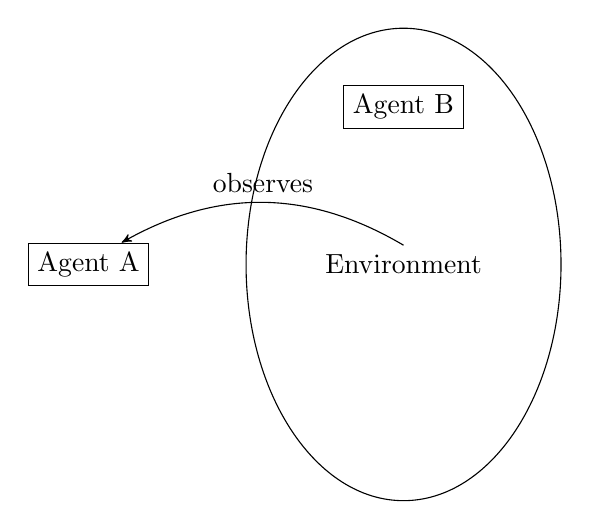
\begin{tikzpicture}[node distance=1cm, auto,]
    % ENVIRONMENT
    \draw (4,0) circle [x radius=2cm, y radius=3cm];

    \node[draw, rectangle] at (4,2) (agentB) {Agent B};
    \node[draw, rectangle] at (0,0) (agentA) {Agent A};
    \node[] at (4,0) (env) {Environment};
    \path[<-,draw, bend left=30]
        (agentA) edge node {observes} (env.north);

    \end{tikzpicture}
    \caption{Agent A indirectly observes B, because he is part of his environment}
    \label{fig:competitiveschema}
\end{figure}



\citeauthor{NG2004Apprentice} demonstrated a technique to teach an agent by letting him imitate the behavior of an expert through inverse reinforcement learning \cite{NG2000InvReinf}. This technique can be used to let reinforcement based agents learn from examples, similar to that of supervised learning methods.



\citeauthor{duan2017one} show another technique of teaching a neural network by providing demonstrations. For this, they perform demonstrations in virtual space, allowing for full observability in a deterministic environment. They explore different architectures and find \emph{Final state with attention} structures to be most effective for their sample tasks
\footnote{This can be reasoned is due to the simple final state of the task which does not require multiple complex intermediary steps for which an LSTM network might have gotten better performance.}.
This work is helpful to understand how an agent can learn from a demonstration in virtual space, adapting itself to achieve the same results. Both this and the work of \citeauthor{NG2004Apprentice} are sketched in \autoref{fig:apprenticeschema}.

\begin{figure}[H]
    \centering
    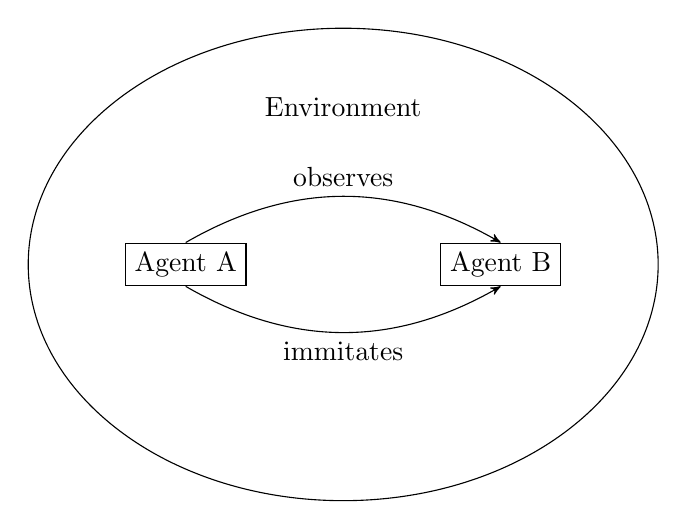
\begin{tikzpicture}[node distance=1cm, auto,]
    % ENVIRONMENT
    \draw (0,0) circle [x radius=4cm, y radius=3cm];

    \node[draw, rectangle] at (2,0) (agentB) {Agent B};
    \node[draw, rectangle] at (-2,0) (agentA) {Agent A};
    \node[] at (0,2) (env) {Environment};
    \path[->, bend left=30]
        (agentA.north) edge node {observes} (agentB.north);
    \path[->, bend right=30]
        (agentA.south) edge node [below]{immitates} (agentB.south);

    \end{tikzpicture}
    \caption{Agent A directly observes B, and learns from him}
    \label{fig:apprenticeschema}
\end{figure}


\citeauthor{jaderberg2017population} show an efficient way of optimizing hyperparameters by letting a population of models exploit each others hyperparameter configurations on-the-fly during learning. For this, a large amount of models are trained in parallel with varying hyperparameters. Those which perform worse copy the values of the hyperparameters of the ones that perform better and continue their training with the new parameters but keeping their previously trained weights.

\begin{figure}[!h]
    \centering
    \includegraphics[width=0.7\textwidth]{population_based_hyperparameters.png}
    \caption{Hyperparameter adoption in population based training \cite{jaderberg2017population}}
    \label{fig:populationtraining}
\end{figure}

\citeauthor{foerster2017learning} show how to allow multiple agents learning in a reinforcement environment to achieve the Nash equilibrium for multiple game theory based games. For this they allow each agent to anticipate another agents learning progress and include this anticipation into their own decision for future action. This work is interesting, because it let's agents understand other agents behavior and then acting upon it. An example is shown in \autoref{fig:anticipatelearning}, where  two cars heading towards each other evade each other based on the "evade to the right" rule. Agent A can anticipate the action of B and therefore increase its utility. By adapting this model, an agent can understand what another agent does.

From this, the utility function can be easily estimated and if it is reasonably close to its own utility function, the same intentions can be assumed, hence it can serve as a role-model if the performance is superior to the agents own performance.

\begin{figure}[H]
    \centering
    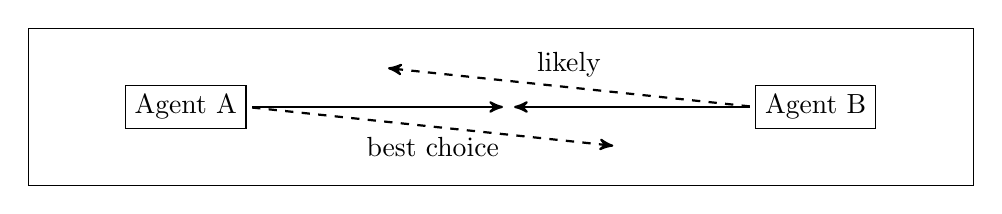
\begin{tikzpicture}[node distance=1cm, auto,]
    % ENVIRONMENT
    \draw (-6,-1) rectangle (6,1);

    \node[draw, rectangle] at (4,0) (agentB) {Agent B};
    \node[draw, rectangle] at (-4,0) (agentA) {Agent A};

    \path[arr] (agentB.west) edge node[below]{} (0.1,0);
    \path[dashedarr] (agentB.west) edge node[above]{likely} (-1.5,0.5);

    \path[arr] (agentA.east) edge node[above]{} (0.1,0);
    \path[dashedarr] (agentA.east) edge node[below]{best choice} (1.5,-0.5);

    \end{tikzpicture}
    \caption{Agent A anticipates move of Agent B and acts accordingly}
    \label{fig:anticipatelearning}
\end{figure}






\newpage
%Bibliography
\bibliographystyle{apalike}
\bibliography{bibliography}

\end{document}
